\chapter{The CMS Detector}\label{sec:detectors}

Since the discovery of the neutron in 30s, humanity's aspiration to understand the most fundamental constituents and laws of the physics have only accelerated.
Discovery of pions, Kaons, and other hadrons from the cosmic rays in 40s, 50s led to understanding of substructure of those particles with Eightfole way of Gell-Mann.
Deep inelastic scattering performed in 60s by the Stanford Linear Accelerator Center (SLAC) confirmed existence of "partons" or "quarks", substructure of those particles.
Observance of J-psi and Upsilon mesons in SLAC and MIT put the third generation fermions in the collection of particles.
Gargamelle bubble chamber in CERN succeeded in detection of muon neutrinos, postulated by Pauli in 30s from the beta decay experiment.
CERN's UA1 and UA2 in 80s confirmed existence of first particles in the electroweak scale, namely the W and Z bosons.
Fermilab's CDF and D0 in 90s confirmed existence of the top quark, the heaviest particle in the SM.
All these discoveries of the most fundamental particles of the universe happened within a half-century.
As much as we appreciate the predecessor physicists for the phenomenal analytic and statistical works, we need to appreciate the evolution of the experimental apparatus as well.
Although simple design of bubble chamber or detection of cosmic rays is still a helpful insight for particle physics research, physicists wanted to create the cosmic and very early phase of the universe on our terra.
Progress from the linear accelerator to TeV scale circular high energy accelerator was achieved by physicists, engineers, and others.
Its pinnacle came with construction fo the LHC, situated in CERN, the home of UA(1-5). 

\begin{figure}[h!]
	\caption{Picture of the CERN complex \cite{CERN}}
  \label{fig:CERN}
  \centering
  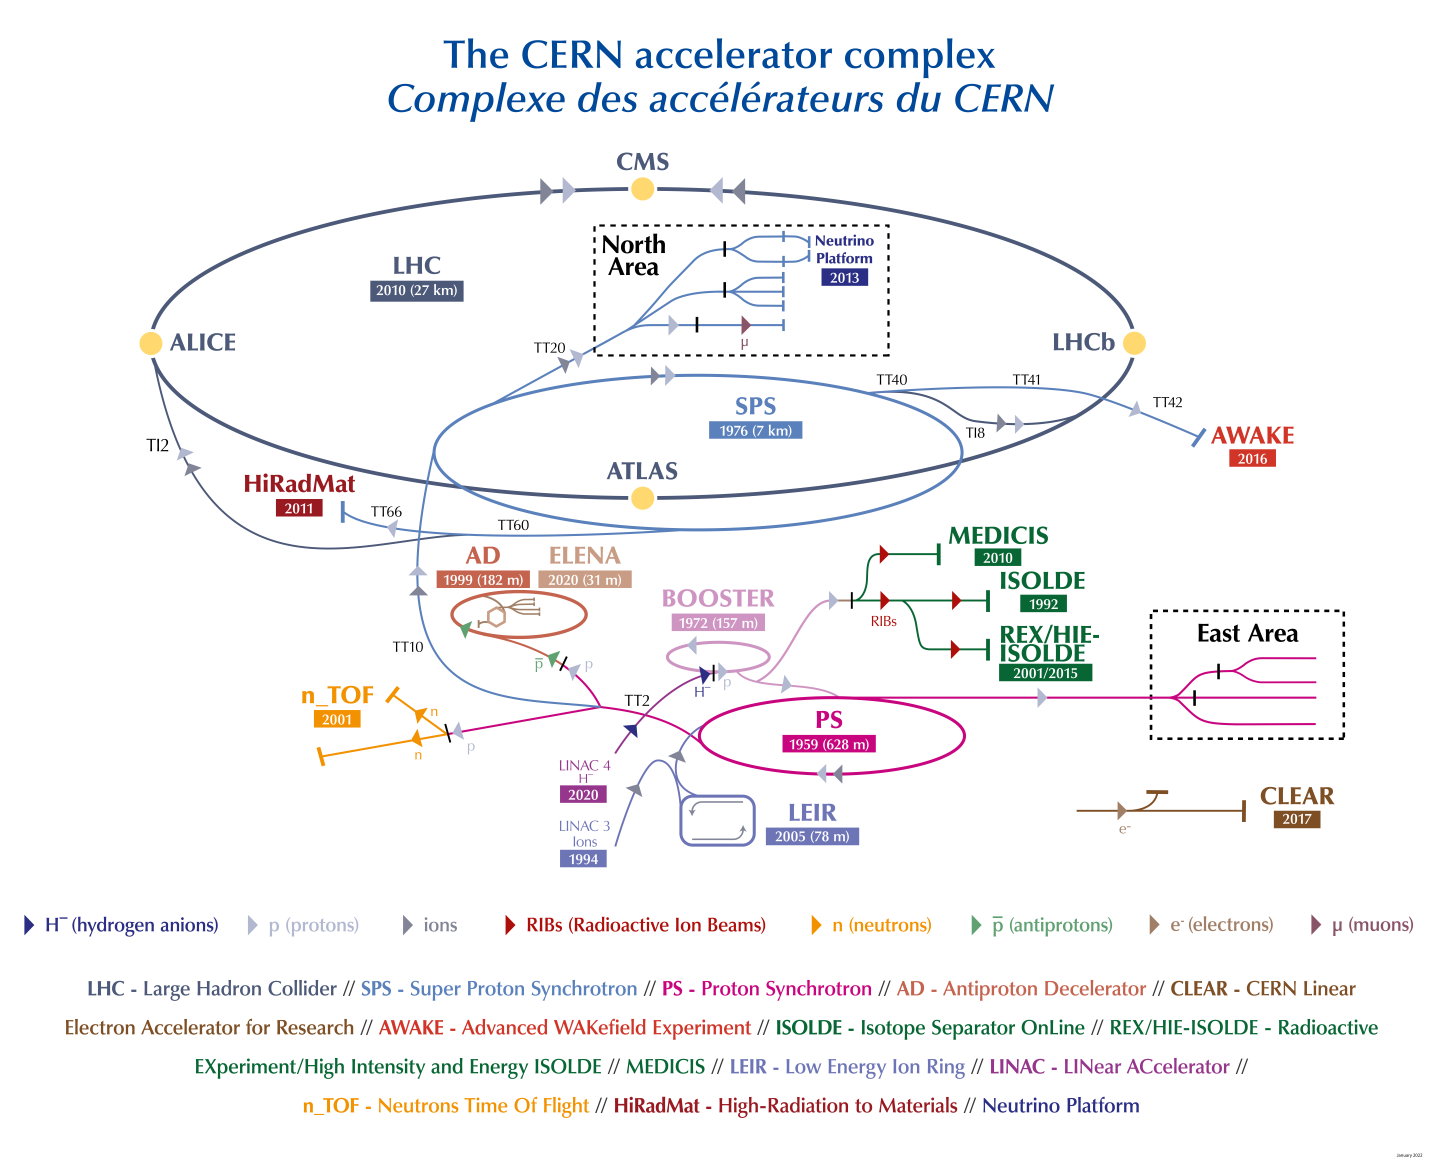
\includegraphics[width=0.9\linewidth]{figs/LHC.png}
\end{figure}


\begin{figure}[h!]
	\caption{Picture of the CMS viewed from the beam direction \cite{det}}
  \label{fig:cms}
  \centering
  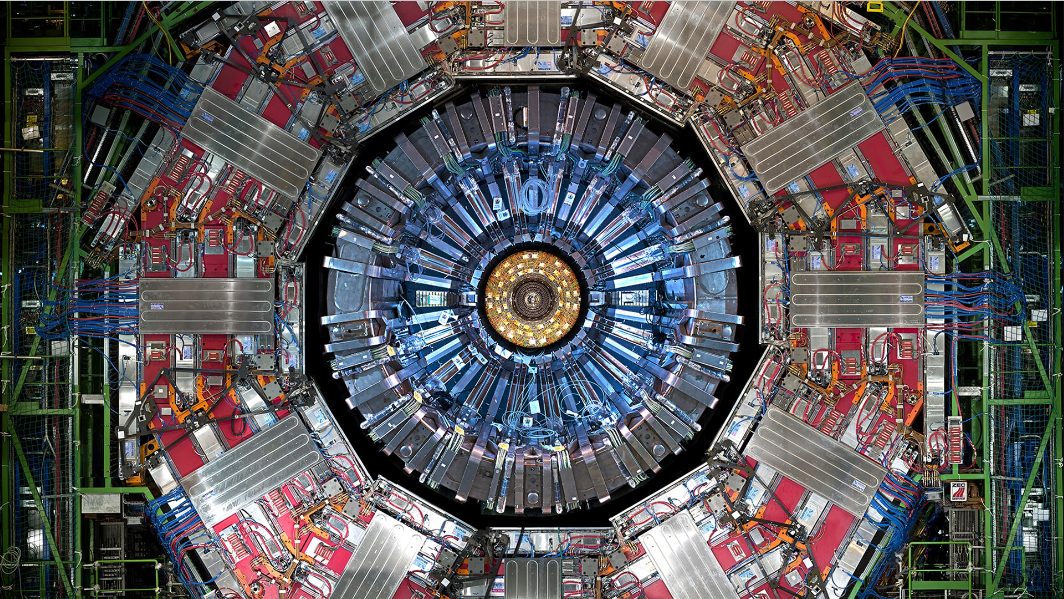
\includegraphics[width=0.9\linewidth]{figs/cms.png}
\end{figure}

\begin{figure}[h!]
	\caption{Cartoon of the CMS with its subpart annotated \cite{xsec}}
  \label{fig:CMS}
  \centering
  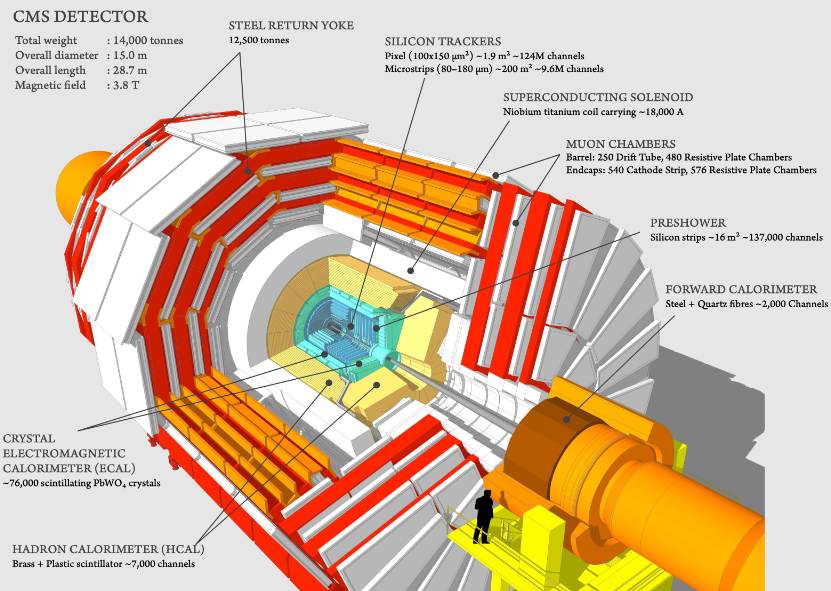
\includegraphics[width=0.87\linewidth]{figs/CMS.png}
\end{figure}


\begin{figure}[h!]
  \caption{Cross-section of the CMS detector as a particle traverses through the apparatus \cite{xsec}}
  \label{fig:cmsxsec}
  \centering
  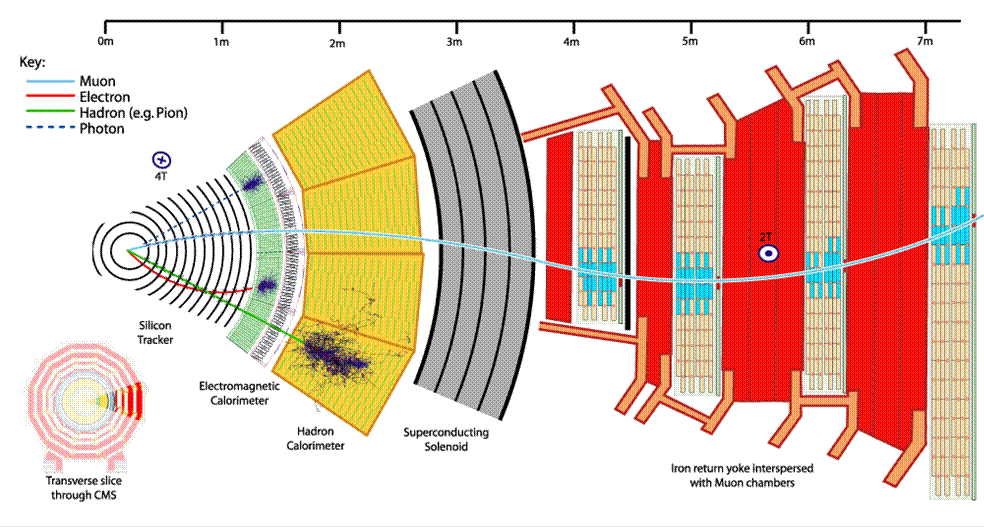
\includegraphics[width=0.87\linewidth]{figs/cmsxsec.png}
\end{figure}

\begin{figure}[h!]
  \caption{Schematic view of the ECAL. \cite{ecal}}
  \label{fig:ECAL}
  \centering
  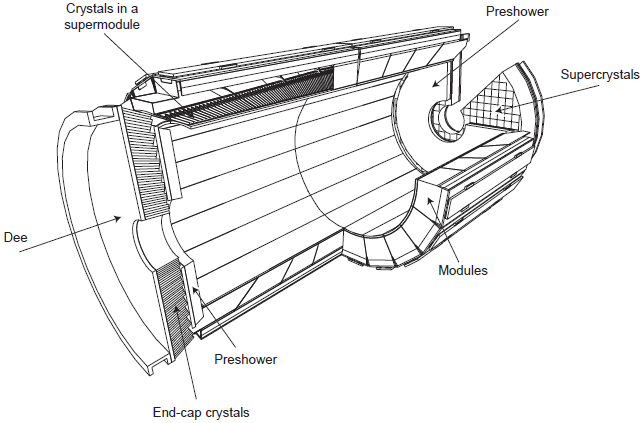
\includegraphics[width=0.87\linewidth]{figs/ECAL.png}
\end{figure}

\begin{figure}[h!]
  \caption{Cross-section of the HCAL in the CMS detector. It shows the Barrel, endcap, front, and outside portion. \cite{hcal}}
  \label{fig:HCAL}
  \centering
  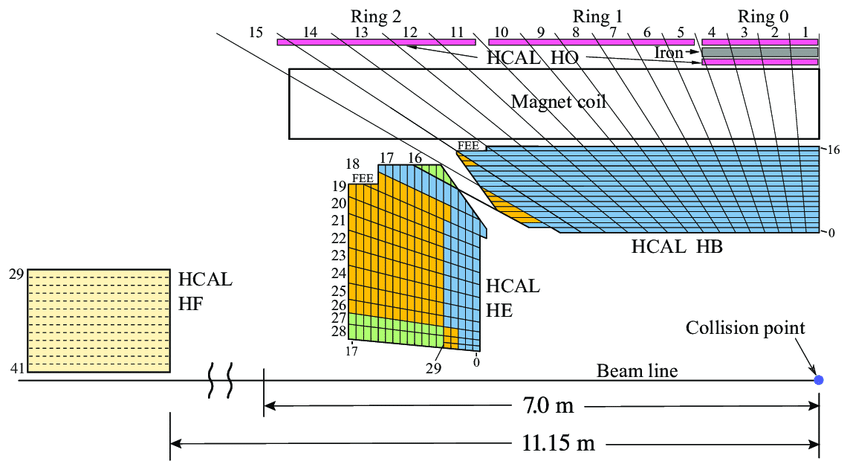
\includegraphics[width=0.87\linewidth]{figs/HCAL.png}
\end{figure}

\begin{figure}[h!]
	\caption{Cross-section of the Muon Chamer in the CMS detector. It shows the 4 layers of the drift tube (DT) cross-section viewed from the z-axis. \cite{det}}
  \label{fig:MC}
  \centering
  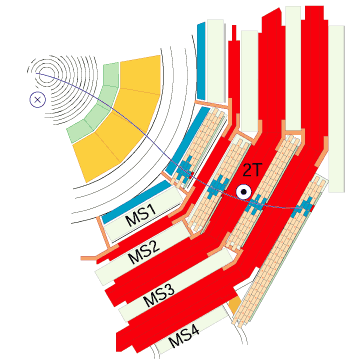
\includegraphics[width=0.4\linewidth]{figs/MCcms.png}
\end{figure}

\begin{figure}[h!]
	\caption{Cross-section of the trackers in the CMS detector. It shows the pixels in the inner tracker for more precise vertexing and the silicon strips on the outer trackers. Silicon strips are tilted with respect to previous layers of strips. \cite{trk}}
  \label{fig:tracker}
  \centering
  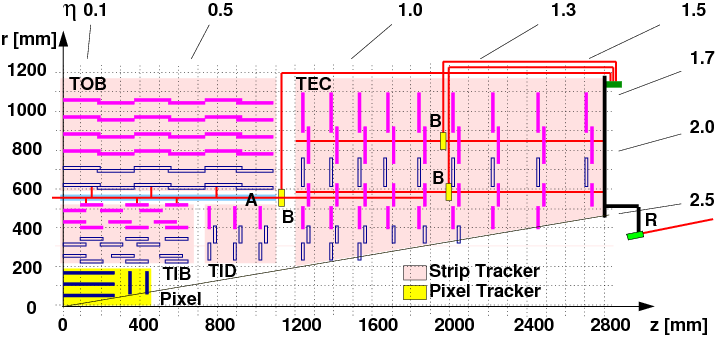
\includegraphics[width=0.9\linewidth]{figs/Tracker.png}
\end{figure}
\section{The LHC and the CMS}
The LHC is the world's largest and highest energy particle collider.
The LHC was built for a decade from 1998 to 2008. 
The construction was completed in collaboration with 100 countries and 10000 scientists around the globe, demostrating the ethos of global cooperation of the physics community and its majestic scale. 
The LHC construction, which costed 5 billion us dollars for its construction , costs 5.5 billion dollars per year for its electric and computing power consumption \cite{LHCweb}.
The LHC is built in a tunnel 328 feet underground at CERN, on the Franco-Swiss border near Annecy, France and  Geneva, Switzerland.
The LHC shoots bunches of protons and lead ions near the speed of light, enabled by the 27 km ring of superconducting magnets with a number of accelerating apparati.
One can infer the LHC name's origin, given that it's 27km long, shoots hadrons of protons, and collide them each other at 0.9997 fraction of the speed of light.

CERN is an acclerator complex, which includes succession of machines with increasingly higher energies. 
Each machine accelerates a beam of particles to a threshold of desired energy, and injects the beam into the next machine in the chain. 
The next machine brings the beam to an even higher energy and repeats the cycle until the entering the LHC. 
The LHC is the last element of this chain, in which the beams reach their highest energies.
The LHC is cooled to 1.9K and maintained at ultrahigh vacuum status.

The goal of LHC was to discover the last remaining piece of the SM, the Higgs boson.
The LHC already succeeded in its primary goal, with discovery of the Higgs boson bo the CMS and ATLAS in July 4th, 2012.
However, the LHC's goal does not stop there. 
As mentioned in \ref{sec:theory}, there still exists several unanswered questions in high energy physics.
LHC wants to address them. It wants to discover the SUSY particles, dark matters, and other exotic particles to help us better understand the most fundamental nature of the universe.

In order to tackle these issues more efficienctly, there are 4 main detectors in the LHC: Compact Muon Solenoid (CMS), A Toroidal LHC Apparatus (ATLAS), A Large Ion Collider Experiment (ALICE), and LHCb.
CMS and ATLAS are general purpose colliders. They were used for the discovery of the Higgs Boson in 2012. They are used for an entire range of the high energy physics, investigating the SUSY particles to dark matter to precision QCD to Lepton Universality.
ALICE is a lead-lead collider, targeting to study a phase of matter called the Quark-Gluon Plasma (QGP). Study of QGP helps us better understand quarks and gluons behavior when they esacape the confinement of the QCD.
Similar research is done in Brookhaven National Laboratory's Pioneering High Energy Nuclear Interaction eXperiment (BNL's PHENIX).
LHCb is a b-factory. It wants to test or challenge "Lepton Universality", claiming that interaction between leptons and a gauge boson measures the same for each lepton. 
Similar research is done in BaBar of SLAC and BelleII of KoEnerugi Kasokuki kenkyu kiko (KEK).
The analysis of this dissertation entirely derives from data obtained in the CMS.
Following subsections detail parts and functions of each part of the CMS.

The CMS consists of 5 main parts: the tracker, the electromagnectic calorimeter (ECAL), the hadronic calorimeter, the superconducting magnet and the Muon chamber.

\subsection{ECAL of the CMS}
Electrons, photons and hadrons will deposit their energies in the calorimeters allowing their energy to be measured. The first calorimeter layer or Electromagnetic Calorimeter (ECAL) is designed to measure the energies of electrons and photons with high precision. Strongly-interacting particles, hadrons, deposit most of their energy in the second layer, the hadron calorimeter (HCAL). Muons and tau leptons deposit only a very small fraction of their energy in the calorimeters, and are detected by consulting also with tracking and muon detector subsystems. Neutrinos escape detection, but their presence can be inferred from an apparent energy imbalance in the interaction.
CMS has a very compact scintillating crystal calorimeter which offers excellent performance for energy resolution since almost all of the energy of electrons and photons is deposited within the crystal volume. The Electromagnetic calorimeter (ECAL) uses about 75,000 lead-tungstate (PbWO4) crystals with coverage in pseudorapidity up to 00000 3.0. The crystals convert energy into light, and the scintillation light is detected by silicon avalanche photodiodes (APDs) in the barrel region and vacuum phototriodes (VPTs) in the endcap region.

A preshower system is installed in front of the endcap ECAL for pi-zero rejection and the detection of photons. This is designed to detect the slightly-overlapping pair of photons from a pi0 decay and to distinguish these from the single shower produced from a single photon interacting with the calorimeter material. .

One of the main physics challenges which sets design requirements for the resolution and efficiency of the EMC is the decay of a low-mass Standard Model Higgs boson into two photons.
\subsection{HCAL of the CMS}
The ECAL is surrounded by a brass/scintillator sampling Hadron Calorimeter (HCAL) with coverage up to 3.0.

The HCAL plays an essential role in the identification and measurement of quarks, gluons, and neutrinos by measuring the energy and direction of jets and of missing transverse energy flow in events. Missing energy forms a crucial signature of new particles, like the supersymmetric partners of quarks and gluons.

The scintillation light is converted by wavelength-shifting (WLS) fibers embedded in the scintillator tiles and channeled to photodetectors via clear fibres. This light is detected by novel photodetectors (hybrid photodiodes, or HPDs) that can provide gain and operate in high axial magnetic fields. While most of the HCAL is contained inside the CMS magnet, there are several additional layers outside the magnet to detect particles from high energy showers.

The central calorimetery is complemented by a "tail-catcher" in the barrel region - ensuring that hadronic showers are sampled with nearly 11 hadronic interaction lengths. This "depth" of the HCAL is needed to contain high-energy jets and also to filter out hadrons from jets involving muons. Accurate measurements of high-energy jets is important for searches for high mass Standard Model and Supersymmetric Higgs bosons.

The hadron calorimeter has both a barrel and endcap component which are sampling calorimeters with 50 mm thick copper absorber plates interleaved with 4 mm thick scintillator sheets. There are also "forward" HCAL's installed at each end of the CMS detector which provide coverage up to a pseudorapidity of 5.0. Here steel absorber plates are used in the harsher radiation environment of the forward systems and hadronic showers are seen by radiation-resistant quartz-fibers. The Cerenkov light emitted in the quartz fibers is detected by conventional photomultiplier tubes. The forward calorimeters ensure full geometric coverage for the measurement of the transverse energy in the event.

Wide rapidity coverage and accurate energy measurements are the main requirements of the hadron calorimetry system as several Higgs modes, as well as other important modes, require good missing transverse energy measurements.
\subsection{The superconducting Magnet  of the CMS}

At the heart of CMS sits a 13-m-long, 5.9 m inner diameter, 12,000 ton, 4 T superconducting solenoid which in part gives CMS its name. The energy stored in the magnet, if liberated, is large enough to melt 18 tons of gold. The CMS magnet system consists of a superconducting coil, the magnet yoke (barrel and endcap), a vacuum tank and ancillaries such as cryogenics, power supplies and process controls. Inside the bore of the magnet sit the inner tracker and the calorimetry, while outside is the flux return system and muon detector.

In order to achieve good momentum resolution with a compact spectrometer it is necessary to have a combination of a high magnetic field and high precision on the spatial resolution and alignment of the detectors. The momentum measurement of charged particles in the detector is based on the bending of their trajectories. The 4T magnetic field also bring benefits for calorimetry - it enables the detection of many isolated electrons produced by the decays of W's, Z's and b quarks. Using these electrons, the CMS crystal electromagnetic calorimeter can be calibrated to an accuracy of a fraction of a percent.

The magnetic flux is returned via a 1.5 m thick saturated iron yoke instrumented with four stations of


\subsection{The Muon Chamber of the CMS}

Muons are expected to provide clean signatures for a wide range of physics processes.
The return field of the solenoid is large enough to saturate 1.5 m of iron, allowing 4 muon "stations" to be interleaved with the iron return yoke plates of the magnet system. This provides a muon system with reconstruction efficiency better than 98\% over the full pseudorapidity range.

Each muon station consists of several layers of aluminum drift tubes (DT) in the barrel region and cathode strip chambers (CSCs) in the endcap region, complemented by resistive plate chambers (RPCs). The muon detectors are arranged in concentric cylinders around the beam line in the barrel region, and in disks perpendicular to the beam line in the endcaps. Muon identification is ensured by the large thickness of the absorber material (iron), which cannot be traversed by particles other than neutrinos and muons. The DT and CSC detectors are used to obtain a precise measurement of the position and thus the momentum of the muons, whereas the RPC chambers are dedicated to providing fast information for the Level-1 trigger.

Muon measurements taken in the muon stations outside the solenoid are used for fast triggering and standalone muon reconstruction, but can also be combined with information from the inner tracking detectors for more precise reconstruction and momentum measurement.

\section{Tracker of the CMS more in detail}

The inner tracker sits around the LHC beampipe. It is cylindrical in shape, of length 5.8 m, and has a diameter of 2.6 m, and consists of 25,000 silicon strip sensors. The system will provide analogue data from ~10 million channels of the microstrip tracker. The CMS tracking system is designed to reconstruct high-pT muons, isolated electrons and hadrons with high momentum resolution and an efficiency better than 98\% in the range 2.5.

The inner-most tracking material consists of 3 layers of silicon pixel detectors which are placed close to the interaction region to improve the measurement of the impact parameter of charged-particle tracks, as well as the position of secondary vertices. In order to deal with high track multiplicities, CMS employs 10 layers of silicon microstrip detectors, which provide the required granularity and precision.

Accurate measurement of secondary vertices is required to study b quark decays - an area of LHC physics which provides rich possibilities to search for new physics interactions. Additionally, detection of particle jets arising from b quark decays, b-tagging, is a very important tool for many other physics studies, from the search of low-mass Higgs bosons to studies of the top quark. Other interactions involving secondary vertex production include the decay of short-lived neutral kaons, KS.

Combined with measurements from the dedicated muon detection system, the tracking system contributes to high resolution muon measurements in CMS.


\section{Trigger of the CMS}
In CMS, a beam spacing of 25 ns, beam crossings occur in the CMS detector at a rate of 40 million per second (40MHz). 
An additional complication is the approximately 25 interactions which occur with each beam crossing - thus giving 1 billion events occurring in the CMS detector every second. 
In order to extract physics from these interactions it is vital to have fast electronics and very good resolution (proton-proton interactions are very messy and produce hundreds or thousands of particle candidates).
because these events occur far too quickly to all be recorded and would take up vast amounts of disk space to store what are, for the majority, uninteresting events, very precise "triggering" is required. 
The CMS Data Acquisition System and Triggering are introduced briefly below.


The Trigger and Data Acquisition System, TriDAS, is designed to select, out of the 1Bn interactions per second produced by 40MHz proton-proton beam crossings, the most interesting hundred or so events for storage and further analysis.

The first level of triggering, Level 1 (L1), is a hardware trigger, using hardware processors to rapidly select or reject events based on information from the ECAL and muon RPCs. Calorimeter triggering is based on a first measurement of energy deposited in the crystals, whereas the muon triggering centers around transverse momentum measurements of muons. The Level 1 trigger reduces the event rate from 40MHz to 100kHz.

An event passing the L1 trigger decision is transmitted to the Data Acquisition System where information from the 16M channels in the CMS subdetector systems is combined by the event builder into a single event. This event is then challenged by the next level of triggering.

The High Level Trigger (HLT) is a software-based trigger which performs a more sophisticated analysis of the event, including applying fast pattern recognition algorithms and event reconstruction. The main reduction factor for events passing the Level 1 triggering is obtained by using tracker information. The HLT decision reduces the event rate to about 100Hz for storage and later offline analysis. This corresponds to about 12 Petabytes of data to be recorded by CMS annually when it is running at design luminosity. The average processing time for the high level trigger is 40ms per event.
